\documentclass[manuscript,screen,review,anonymous=false]{acmart}
\usepackage[export]{adjustbox}

% https://scf.acm.org/2021/submissions.html

% \usepackage{tabularx}
% \usepackage{fancyvrb}
% \DefineVerbatimEnvironment{verbatim}{Verbatim}{xleftmargin=.25in}
% \DefineVerbatimEnvironment{Code}{BVerbatim}{baseline=t}
\usepackage{subcaption}
\usepackage{fancyvrb}
\usepackage{fvextra}
\usepackage{alltt}

\setcopyright{acmcopyright}
\copyrightyear{2021}
\acmYear{2021}
\acmDOI{10.1145/1122445.1122456}

\acmConference[SCF '18]{SCF '18: ACM Symposium on Computational Fabrication}{October 27--28, 2021}{Online}
\acmBooktitle{SCF '18: ACM Symposium on Computation Fabrication, October 27--28, 2021, Online}
\acmPrice{15.00}
\acmISBN{978-1-4503-XXXX-X/18/06}

%%\acmSubmissionID{123-A56-BU3}

\begin{document}

\title{Supporting Algorithms and Aesthetics in Computational Making}

\author{Chris Johnson}
\email{johns8cr@jmu.edu}
\affiliation{%
  \institution{James Madison University}
  \city{Harrisonburg}
  \state{Virginia}
  \country{USA}
}

\renewcommand{\shortauthors}{Johnson}

\begin{abstract}
Designers interact with digital representations of objects in two different ways. With direct manipulation, the designer transforms an object by clicking and dragging on the canvas with a mouse or other pointing device. With indirect manipulation, the designer writes code that generates the object when the code is executed. Tools often support only one of these manipulation styles, which reinforces the false dichotomy separating artists from programmers and aesthetics from algorithms. In this paper, we present Twoville, a design tool that embraces both manipulation styles simultaneously. Programmer-artists use both their algorithmic and aesthetic senses in Twoville to create design files for 2D fabrication devices. Edits made in the code editor change the object in the canvas, and edits made in the canvas change the code that produced the object. We describe Twoville and offer an informal and formative evaluation of it through the eyes of a young beta tester.

\end{abstract}

%% The code below is generated by the tool at http://dl.acm.org/ccs.cfm.
\begin{CCSXML}
<ccs2012>
   <concept>
       <concept_id>10010147.10010371.10010387</concept_id>
       <concept_desc>Computing methodologies~Graphics systems and interfaces</concept_desc>
       <concept_significance>500</concept_significance>
       </concept>
   <concept>
       <concept_id>10003120.10003121.10003128</concept_id>
       <concept_desc>Human-centered computing~Interaction techniques</concept_desc>
       <concept_significance>500</concept_significance>
       </concept>
 </ccs2012>
\end{CCSXML}

\ccsdesc[500]{Computing methodologies~Graphics systems and interfaces}
\ccsdesc[500]{Human-centered computing~Interaction techniques}

%%
%% Keywords. The author(s) should pick words that accurately describe
%% the work being presented. Separate the keywords with commas.
\keywords{computational making, direct manipulation, bidirectional editing}

\maketitle

\section{Introduction}
\section{Introduction}
\label{section:introduction}

% Twoville is a programming language and development environment for composing vector graphics files for tools like vinyl and laser cutters and pen plotters. Its users write code to generate, transform, and combine geometric shapes that determine the cutting or drawing path of these fabrication tools. The output of a program is a physical artifact that has a life beyond its digital roots.

In our experience, many educational makerspace efforts start with the best of intentions but degenerate into passive consumerism. Rather than flexing their own creative muscles, users download and fabricate designs made by others. One explanation for this behavior is that designing artifacts takes time, accessible tools, and trained educators, none of which may be available in an educational setting constrained by inflexible curriculum and inadequate resources. Grants provide money for equipment and supplies, but little else. The availability of fabrication equipment has helped democratize the physical manufacturing of artifacts, but designing one's own artifacts is still difficult.

Twoville is our attempt to make computation and fabrication more accessible for students in our local community. It is a programming environment for creating vector graphics files that can be fed into 2D fabrication tools like vinyl and laser cutters, pen plotters, and embroidery machines. The software runs in the browser and is open source. Its primary audience is learners in educational makerspaces. It offers a low barrier to entry so that novices may quickly fabricate something of their own design. At the same time, the scope of objects that may be designed is expansive. Writing Twoville programs is a cognitive process in which learners draw upon computational and mathematical knowledge. It is our hope that teachers can incorporate Twoville into their classroom activities and still meet curricular expectations.

As we've developed the language, we have come to the unoriginal conclusion that not all design work can be effectively programmed. Code is an indirect interface, and artists often want more direct control driven by aesthetic feel. Therefore, we provide an interface that supports bidirectional editing. The programmer-artist can edit the code, which updates the output, or edit the output, which updates the code. Objects may be shaped both algorithmically and through mouse-based direct manipulation of parameters.

This experience report is an introduction to the Twoville language and development environment. In Section~\ref{section:related_work}, we examine prior work that Twoville builds on. In Section~\ref{section:language}, we describe the language and the motivations behind our design choices. In Section~\ref{section:case_study}, we share an informal evaluation of Twoville by examining it through the eyes of a young beta tester.


\section{Related Work}
\section{Related Work}
\label{section:related_work}

The prior work that has informed the development of Twoville can be clustered into three main categories: computational making, programming languages for fabrication, and direct manipulation in user interfaces.

\subsection{Computational Making}
Rode et al.~\cite{rode15ctcm} define \textit{computational making} as the integration of computational thinking and several making-related activities and skills, namely ``aesthetics, creativity, construction, visualizing multiple representations, and understanding materials.'' Learners who engage in computational making integrate different kinds of thinking, including virtual and physical, algorithmic and aesthetic, and abstract and concrete.

Jacobs and Buechley~\cite{jacobs13codeable} discuss several advantages that computational design systems provide, including precision and automation, generativity and randomness, and parameterization.

Chytas et al.~\cite{chytas2018learning} held a series of workshops on parametric design and analyzed the participants' OpenSCAD~\cite{openscad} and BlocksCAD~\cite{blockscad} programs to understand the how parametric design contributes to the learning of programming. Half of the projects did not include any loops, and very few used conditional statements. These low frequencies can be explained to some degree by a bias toward novice programmers in an experimental environment. In our experience with Twoville, we have also found that many interesting objects can be made without flow control. Not every programming language feature is important in the initial stages of computational making, which we view positively.

A considerable number of projects have engaged learners in computational making via programmable textiles~\cite{rode15ctcm,buechley10lilypad,kafai14crafts}. In some of these projects, the constructed object is made of two distinct elements: a programmable embedded system and a physical housing, like a garment of clothing or a puppet. With Twoville, the physical artifact is itself the product of the computation. Once fabricated, the object is no longer tied to a computer.

Other textile projects allow designers to program the designs themselves. Yu and McCann~\cite{yu2020coupling} describe an interface that allows users to see the connection between lines of code and their associated stitches in a visualization of a programmed knitting pattern. Twoville offers a similar linked editor. When the cursor is placed in the code, the corresponding component of a shape is highlighted in the canvas and can be edited visually.

\subsection{Programmatic Fabrication}
A growing but small number of programming environments have been developed for creating physical artifacts. Many are research projects, and only a few have had public releases.

Some tools confine the design space to two dimensions. The FlatCAD system of Johnson~\cite{johnson08flat}, for example, is used to programmatically trace out flat shapes that can be laser-cut and assembled into more complex objects. Turbak et al.~\cite{turbak12tangible} describe two blocks languages for generating design files that can be cut or engraved with laser cutters. Other tools support fabrication in three dimensions. Beetleblocks~\cite{koschitz12exploring} and Madeup~\cite{johnson17toward} both generate printable 3D models using imperative languages inspired by Logo. OpenSCAD and BlocksCAD provide declarative languages in which complex models are composed using simpler primitives.

Johnson~\cite{johnson08flat} observes that programming is not always the most natural means of interacting with a design. A more versatile design tool would additionally allow sketching and direct manipulation. Twoville is a two-dimensional design tool that supports both direct manipulation on the canvas and indirect manipulation through code.

\subsection{Direct Manipulation}
Schneiderman~\cite{shneiderman19931} explored direct manipulation across a diverse set of professional domains and summarized it as an interactive mode of editing where actions are rapidly executed, immediately observable, and easily reversed. Physically interacting with the system produces direct, visual results. These principles of interactive design have since been applied to integrated development environments (IDEs) to make the generation and editing of code more intuitive.

Adam et al.~\cite{adam19dm} compared direct manipulation interfaces to text interfaces in a study of novice programmers. Half of the subjects used a tool that generated code as they directly interacted with the data. The other half used a text editor. The direction manipulation group solved fewer programming exercises than the text group but achieved higher scores on the exercises they did complete. In exercises involving conditionals and repetition, each editing mode had its advantages. Adam et al. hypothesize that an ideal interface would combine both methods of input.

Hundhausen et al.~\cite{hundhausen09dm} investigated whether direct manipulation makes programming more accessible than text and whether the knowledge acquired using a direct manipulation interface to program transfers to a text interface. They found that students in an introductory programming course who used direct manipulation completed coding tasks more accurately and quickly than students using text. Further, when this experimental group switched to text for the final exercise, they continued to outperform the control group. \textit{Dual-coding theory}~\cite{clark1991dual}, which states that knowledge is strengthened when it is encoded in multiple ways, may explain this positive result.

The CapStudio project of Fukahori et al.~\cite{fukahori14capstudio} is a game editor that allows game developers to write source code and directly manipulate the game objects in the visual display. They label a source code change that propagates to the visual display a {\em forward edit}, and a change in the visual display that propagates to the source code a {\em backward edit}. We apply the term {\em bidirectional editor} to Twoville.

The Sketch-and-Sketch project of Chugh et al.~\cite{chugh16dm} heavily inspires our work on Twoville. Both projects are environments for indirectly coding and directly manipulating vector graphics designs. When a Sketch-and-Sketch program is evaluated, each visual property of a shape---like size and position---is stored with a \textit{trace}, which is an unevaluated representation of the expression that generated it. This expression is composed of one or more parameters. When the designer manipulates the shape using the mouse, the new value of the property and the source expression are used to solve for one of the parameters. The new value replaces the old value in the source code. Twoville differs in several ways from Sketch-and-Sketch. It is an imperative language rather than a functional language, and it relies on simpler heuristics to update ambiguous or complex expressions. These adaptations were intentionally chosen to cater to an audience of computational makers and young learners.


% \section{Language}
% \label{section:language}

Twoville is a browser-based vector graphics editor. Its interface is composed of a code editor and a drawing canvas, as shown in Figure~\ref{figure:droplet}. The Twoville programming language is a textual language whose syntax is inspired by Python and Ruby. It supports variables, mathematical and logical operators, procedural abstraction, conditional statements, iteration, and lists.

We chose to implement a custom language instead of adopting a mainstream language because supporting direct manipulation in a linked interface requires the tool to have considerable understanding and control of a programmer-artist's source code. A mainstream language has more features than we want to support in a tool designed for learners. 

Some of the syntax design choices warrant an explanation. In particular, few function calls allow parameters. This is a deliberate choice. In many languages, parameters are an ordered list of naked expressions. A parameter's significance is determined merely by its position, and tacit knowledge of a function's interface is required to understand its significance. Languages that support named parameters make the significance explicit. However, named parameters tend to lengthen the lines in the source code. The devices typically found in classrooms tend to have small screens, so the text doesn't fit in the editor, which leads to horizontal overflow or wrapping. Neither makes for a good user experience.

The ergonomic situation of our primary audience has therefore led us to a mostly-parameterless syntax. In a traditional language, lines 5--8 in Figure~\ref{figure:droplet} would be expressed as
\begin{verbatim}
cubic([24, 30], [45, 65], [20, 58])
\end{verbatim}
In a language with named parameters, this might be expressed as
\begin{verbatim}
cubic(position = [24, 30], control1 = [45, 65], control2 = [20, 58])
\end{verbatim}
In Twoville, each parameter is treated as a property whose value must be set on the object returned from the function. The \verb=with= block makes this object the target of the property assignments that follow. This way of structuring function calls consumes more vertical space than the alternatives, but the significance of the properties is explicit and the code is less likely to overflow horizontally.

\begin{figure}
\centering
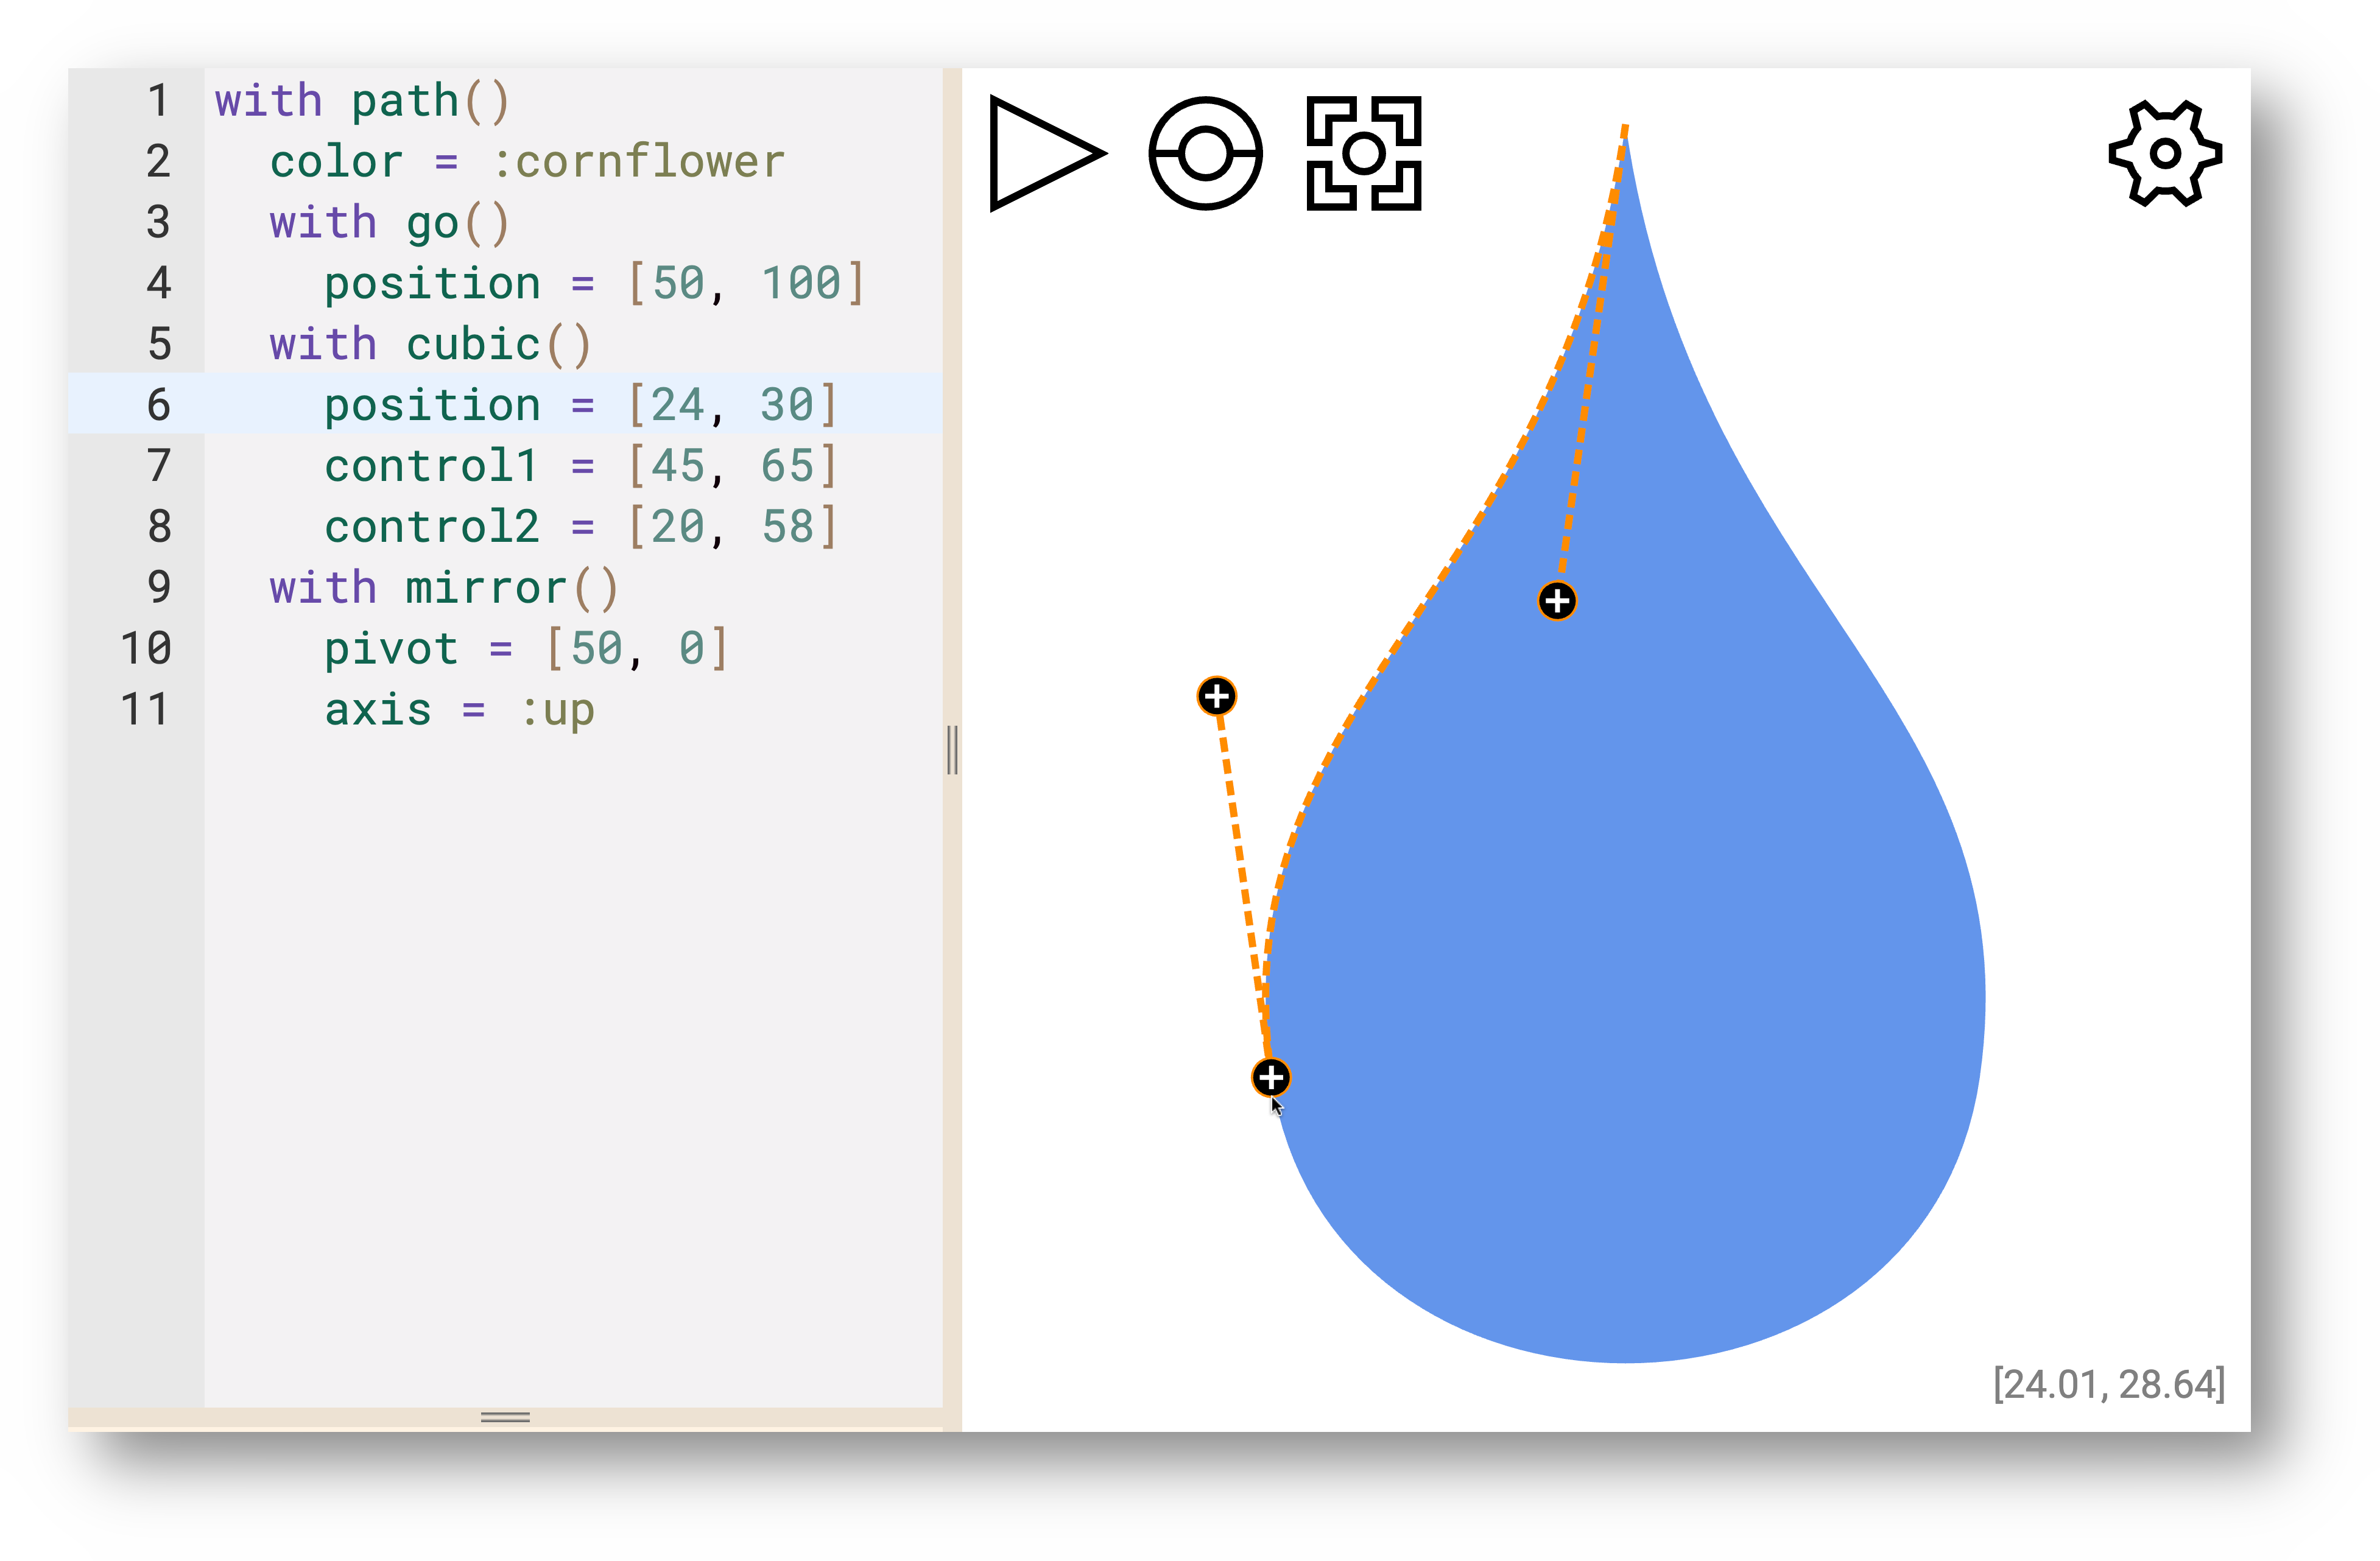
\includegraphics[width=\linewidth]{pixels/droplet}
\caption{A shape composed in piecewise fashion using using line segments and arcs.}
\label{figure:droplet}
\end{figure}


% \section{Bidirectional Editing}
% \input{bidirectional}

% \section{Case Studies}
% \input{case_studies}

% \section{Conclusion}
% \section{Conclusion}

We have introduced Twoville, a new platform for computational making. The bidirectional editor allows programmer-artists to shape structures both algorithmically and aesthetically. The digital design is exported as an SVG file and loaded in a fabrication tool, which cuts or engraves it in physical material.

Our primary goal in building Twoville is to use it as a vehicle for empowering young learners in makerspaces and schools to apply the mathematics and computation that they are learning to creative physical construction. The next steps for us in this process are to form partnerships with teachers and media specialists and to develop lessons and exercises that we can use in classrooms and outreaches. At the time of this writing, we are using Twoville in a summer camp, and we have plans to use it in a weekly after-school program this next academic year.


\bibliographystyle{ACM-Reference-Format}
\bibliography{papers}

\end{document}
\endinput
